\chapter{Resultados e Discussão}
\label{cap:exemplos}

% figuras estão no subdiretório "figuras/" dentro deste capítulo
\graphicspath{{\currfiledir/figuras/}}

%=====================================================

\section{Acumulador / Células}

    É o conjunto de todas as células de bateria ou supercapacitores que armazenam energia elétrica para ser usada no sistema de tração (\textit{Tractive System – TS}), no veículo elétrico, ou no sistema de alta tensão (\textit{High Voltage System – HVS}), na microrrede. Não existem muitos requerimentos nessa parte, principalmente no sistema da microrrede. Já no veículo elétrico, a tensão máxima é limitada em 600 V.

    A escolha do modelo de célula a ser utilizada se iniciou com uma pesquisa de fabricantes, sendo LG, Samsung e Panasonic/Sanyo as mais conhecidas e disponíveis. Apenas células cilíndricas são usadas, sua preferência é justificada pelo uso facilitado, a não necessidade de um container com controle de pressão, a presença de dispositivos de proteção internos, além da experiência prévia no uso de células cilíndricas em projetos anteriores. Uma lista das melhores células dessas fabricantes foi feita.

    Características do \textit{datasheet} foram observadas ao montar o gráfico da figura \ref{fig:ragone-celulas}, comparando a energia específica e potência específica das células. É possível ver uma clara distinção entre células de alta potência e células de alta energia, sendo as de alta potência na parte mais à direita do gráfico e as de alta energia na parte superior.

    \begin{figure}[!htb]
        \centering
        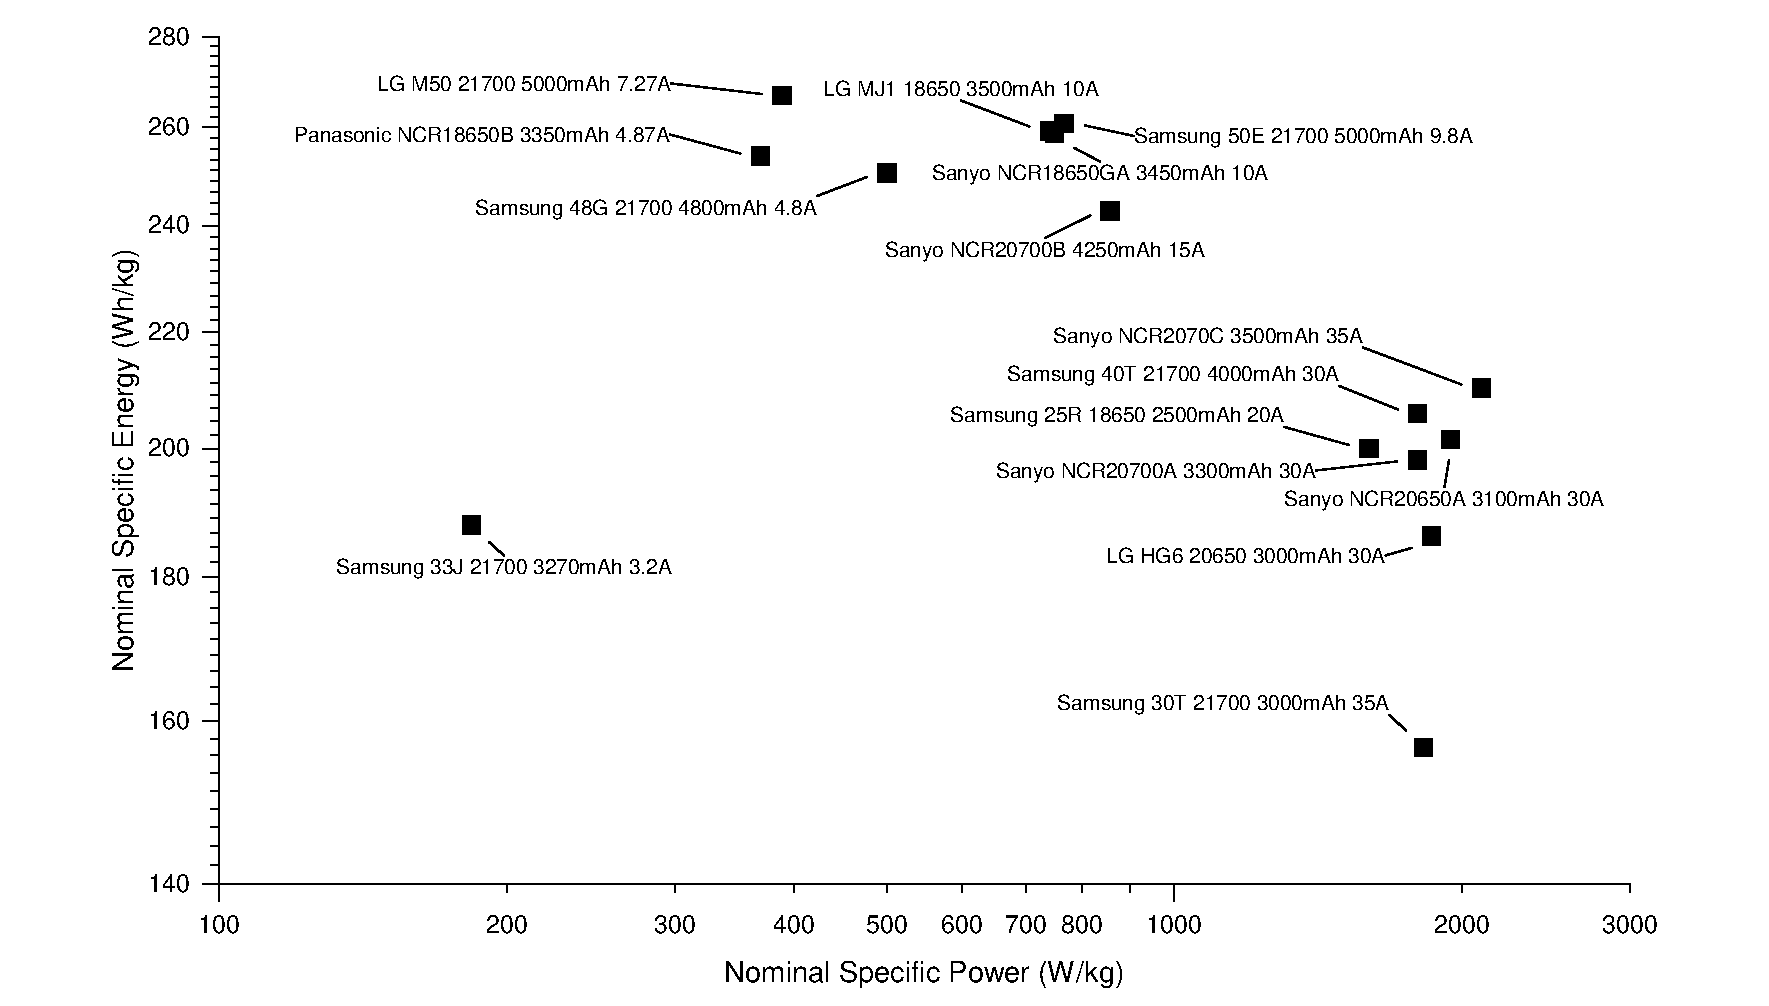
\includegraphics[width=\linewidth]{ragone-celulas.pdf}
        \caption{Comparação de dados do datasheet dos modelos de células analisados.}
        \label{fig:ragone-celulas}
    \end{figure}

    Desses modelos apresentados acima, os 11 mais promissores foram adquiridos para o desenvolvimento dos testes. Estes foram feitos seguindo os principais padrões internacionais (como a IEC 62660-1:2010). 

    Inicialmente é realizado um teste de pré-condicionamento (\textit{Preconditioning Test}) para verificar se a capacidade da célula se mantém constante em testes seguidos, além de preparar a célula para os testes seguintes. Após isso é realizado o ciclo padrão (\textit{Standard Cycle}) com o objetivo de verificar a capacidade nominal da célula. O teste de capacidade (\textit{Capacity Test}) é realizado, em seguida, para se obter o valor da capacidade em função da corrente de teste (tabela \ref{tab:40T-testeresultados-cap} e figura \ref{fig:40T-testegraf-cap}). Após isso, é feito o teste de ciclo de baixa corrente (\textit{Low C-rate Cycle}), que tem por objetivo obter o valor da tensão de circuito aberto em relação ao estado de carga (figura \ref{fig:40T-testegraf-ocv}). Por último, o teste de impedância eletroquímica (\textit{Electrochemical Impedance Spectroscopy – EIS}), que tem por objetivo monitorar a relação entre a impedância da célula e seu estado de carga, durante os ciclos de carga e descarga (figura \ref{fig:40T-testegrafs-imp}).

    \begin{table}[!htp]
        \centering
        \caption{Resultados do teste da capacidade da célula Samsung 40T.}
        \label{tab:40T-testeresultados-cap}
        \begin{tabular}{lccc}
           \hline
           \multicolumn{1}{c}{}& Tensão média & Carga & Energia \\
           \hline
           0,2C & 3,646 V & 3,970 Ah & 14,483 Wh \\
           0,5C & 3,634 V & 3,891 Ah & 14,145 Wh \\
           1C   & 3,599 V & 3,842 Ah & 13,833 Wh \\
           5C   & 3,441 V & 3,874 Ah & 13,216 Wh \\
           \hline
        \end{tabular}
    \end{table}
    
    \begin{figure}[!htb]
    \centering
        \begin{subfigure}{0.48\linewidth}
            \centering
            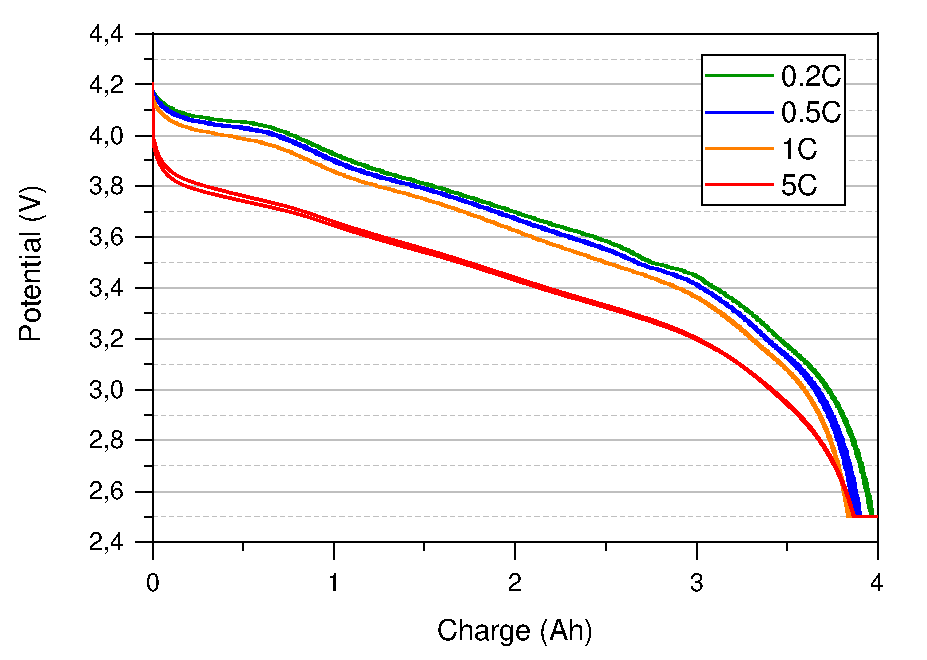
\includegraphics[width=\linewidth]{40T-testegraf-cap.pdf}
            \caption{Capacidade em relação a carga.}
            \label{fig:40T-testegraf-cap}
        \end{subfigure}
        \hspace*{\fill}
        \begin{subfigure}{0.48\linewidth}
            \centering
            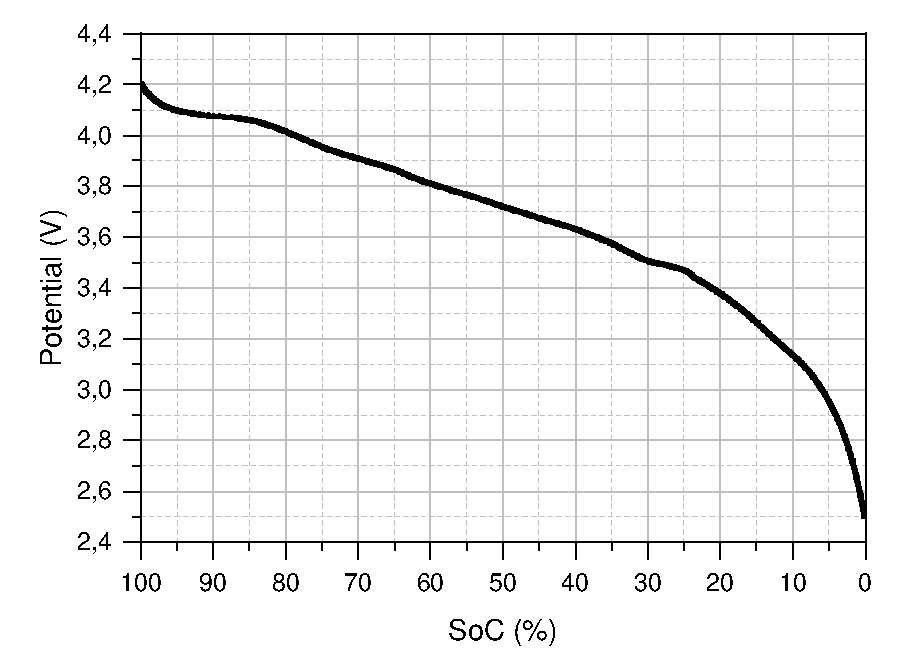
\includegraphics[width=\linewidth]{40T-testegraf-ocv.pdf}
            \caption{Tensão de circuito aberto em relação ao estado de carga (SoC).}
            \label{fig:40T-testegraf-ocv}
        \end{subfigure}
    \caption{Graficos dos testes da célula Samsung 40T.}
    \label{fig:40T-testegrafs-cap}
    \end{figure}
     
    \begin{figure}[!htb]
        \centering
            \begin{subfigure}{0.48\linewidth}
                \centering
                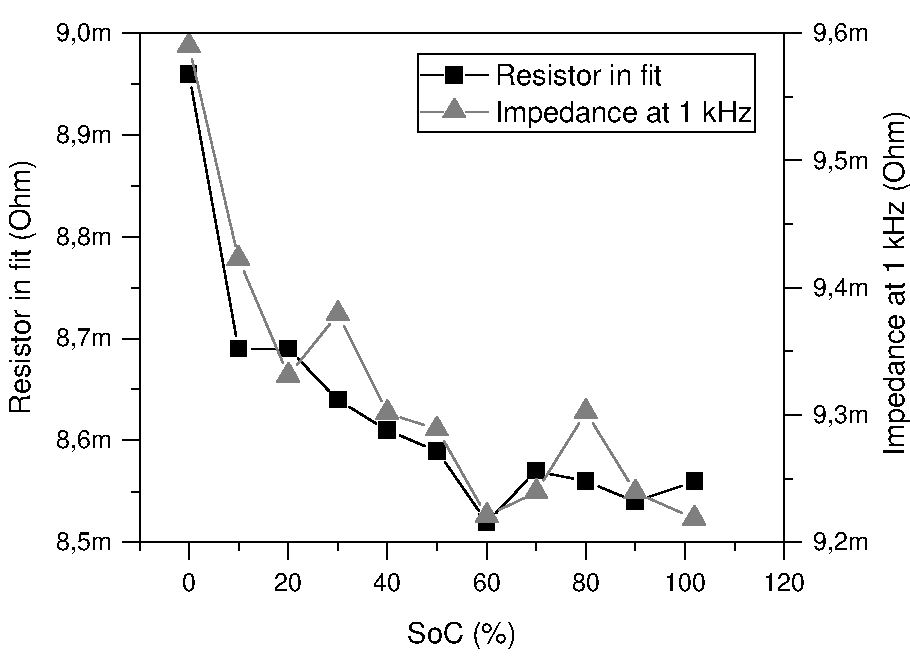
\includegraphics[width=\linewidth]{40T-testegraf-imc.pdf}
                \caption{Carga.}
                \label{fig:40T-testegraf-imc}
            \end{subfigure}
            \hspace*{\fill}
            \begin{subfigure}{0.48\linewidth}
                \centering
                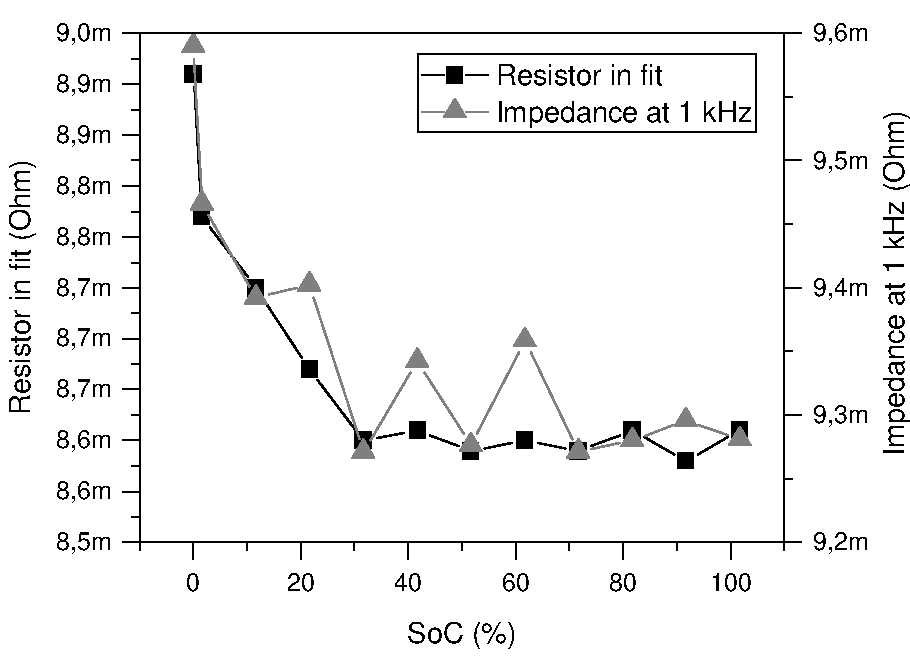
\includegraphics[width=\linewidth]{40T-testegraf-imd.pdf}
                \caption{Descarga.}
                \label{fig:40T-testegraf-imd}
            \end{subfigure}
        \caption{Graficos dos testes de impedância em relação ao estado de carga (SoC) da célula Samsung 40T.}
        \label{fig:40T-testegrafs-imp}
    \end{figure}

    Apesar de todas as células de testes terem sido adquiridas, não foi possível realizar todos os testes previstos em razão da pandemia de COVID-19. Sendo que foi possível a coleta de dados de apenas uma unidade da célula Samsung 40T. Desta forma, infelizmente, não foi possível que houvessem dados reais de teste para o embasamento da escolha das células, assim, serão usados apenas dados do datasheet. Apesar de não ter sido possível a comparação com dados dos demais modelos de célula, os dados abaixo da célula Samsung 40T foram usados para a simulações da célula.

    Com os dados de datasheet já comparados anteriormente, foi observado que a célula Samsung 40T é a que apresenta o melhor desempenho de potência com uma energia satisfatória e a Samsung 50E apresenta o melhor desempenho de energia com uma potência satisfatória, por isso, foram escolhidas para serem utilizadas nos dois acumuladores sendo desenvolvidos: 40T para o veículo elétrico e 50E para a microrrede. 

    Após as células terem sido escolhidas foi feito o dimensionamento do acumulador, ou seja, a quantidade de células em série e paralelo. Inicialmente os valores de referência foram definidos, para a tensão, energia e corrente (tabela \ref{tab:acc-desejado}). As tensões máximas foram definidas para estarem próximas dos máximos permitidos pelos sistemas nas quais elas seriam conectadas: 600 V nominal e 800 V máximo para o conversor CC-CC da microrrede, 550 V máximo para o motor do veículo elétrico. Além disso levando em consideração a segurança de quem for realizar manutenção e operação dos sistemas, a tensão da microrrede será limitada em 600 V. A tensão máxima do veículo foi também limitada abaixo de 500 V para que os componentes de potência utilizados em sistemas de segurança sejam mais simples e por consequência mais leves. A corrente máxima, no veículo, de 170 A foi definida para que seja possível ter um bom desempenho de potência, para garantir uma aceleração rápida em qualquer circunstância. A energia total do sistema da microrrede de 20 kWh foi um requerimento apresentado pelo sistema e previamente calculado em outros estudos. A energia do veículo elétrico, de 6kWh, foi estimada para que seja possível andar por volta de 20 km com uma carga, que seria o equivalente à prova mais longa da competição. Para isso foram feitas simulações do desempenho do sistema de tração em conjunto com o restante do carro.

    \begin{table}[!htp]
        \centering
        \caption{Valores desejados para o dimensionamento dos sistemas.}
        \label{tab:acc-desejado}
        \begin{tabular}{lcc}
            \hline
            Sistema                                      & Microrrede    & Veículo elétrico  \\
            Energia [Wh]                                 & 20000 Wh      & 6000 Wh           \\
            Corrente máxima [A]                          & 120,00 A      & 170,00 A          \\
            Tensão máxima desejada [V]                   & 600 V         & 480 V             \\
            Tensão máxima do sistema conectado [V]       & 800 V         & 550 V             \\
            Tensão máxima permitida (regulamento) [V]    & --            & 600 V             \\
            \hline
        \end{tabular}
    \end{table}

    Com esses dados foi possível calcular a quantidade de células necessária. Inicialmente calculando a quantidade de células em série, apenas dividindo a tensão máxima desejada pela tensão máxima de uma célula. Esses valores foram, então, arredondados para melhor encaixarem na montagem final. Após isso, a quantidade de células em paralelo desejada foi calculada de duas formas: a partir da corrente (potência) e a partir da energia. Pode-se ver que em ambos os casos esses dois valores acabam sendo parecidos, refletindo a boa escolha da célula para as necessidades do sistema. Novamente, foi arredondado o valor das células em paralelo. Na tabela \ref{tab:acc-projeto} é possível ver todas as características calculadas do acumulador.

    \begin{table}[!htp]
        \centering
        \caption{Características do acumulador.}
        \label{tab:acc-projeto}
        \begin{tabular}{lcc}
            \hline
            Sistema                                         & Microrrede    & Veículo elétrico  \\
            Fabricante                                      & Samsung       & Samsung           \\
            Modelo                                          & INR21700-50E  & INR21700-40T      \\
            Células em série (calculado)                    & 142,86        & 114,29            \\
            Células em série (arredondado)                  & 144           & 115               \\
            Células em paralelo (calculado para potência)   & 8,16          & 3,78              \\
            Células em paralelo (calculado para energia)    & 7,72          & 3,62              \\
            Células em paralelo (arredondado)               & 8             & 4                 \\
            Número total de células                         & 1152          & 460               \\
            Capacidade nominal [mAh]                        & 40 Ah         & 16 Ah             \\
            Corrente nominal de descarga contínua [A]       & 7,84 A        & 3,20 A            \\
            Corrente máxima de descarga contínua [A]        & 117,60 A      & 180,00 A          \\
            Corrente nominal de carga contínua [A]          & 19,60 A       & 8,00 A            \\
            Corrente máxima de carga contínua [A]           & 39,20 A       & 24,00 A           \\
            Corrente de fim de carga (Cut-off) [mA]         & 784 mA        & 400 mA            \\
            Corrente de curto circuito [A]                  & 822,86 A      & 1200,00 A         \\
            Tensão máxima [V]                               & 604,80 V      & 483,00 V          \\
            Tensão nominal [V]                              & 518,40 V      & 414,00 V          \\
            Tensão mínima [V]                               & 360,00 V      & 287,50 V          \\
            Impedância AC máxima em 1kHz [m$\Omega$]        & 4,38 m$\Omega$& 3,00 m$\Omega$    \\
            Potência nominal [W]                            & 4,064 kW      & 1,325 kW          \\
            Potência nominal (corrente máxima) [W]          & 60,964 kW     & 74,520 kW         \\
            Potência máxima [W]                             & 71,124 kW     & 86,940 kW         \\
            Energia nominal [Wh]                            & 20736 Wh      & 6624 Wh           \\
            Volume [L]                                      & 26,2679 L     & 11,4365 L         \\
            Massa [g]                                       & 79,49 kg      & 32,20 kg          \\
            \hline
        \end{tabular}
    \end{table}

%=====================================================

\section{Segmentos}

    São subgrupos de células de bateria que podem ser isoladas entre si, de forma que atendem as especificações do item EV.4.1.2 do regulamento para Formula SAE. É um sistema somente do veículo elétrico, não se deve confundir os segmentos do veículo elétrico com os módulos do acumulador da microrrede, justamente pelas especificidades desse regulamento para o uso em veículos. É usado como forma de proteção quando manutenção do sistema HV é necessária. Além disso permite ainda uma modularidade do sistema, semelhante à função dos módulos. Têm a tensão máxima limitada em 120 V e a energia máxima limitada em 6 MJ por segmento. O acumulador do veículo elétrico foi então separado em 5 segmentos, cada um com 23 células em série e 96,6 V de tensão máxima, com a energia máxima total de 5,56 MJ. 
    
%=====================================================

\section{Container}

    O container é o invólucro de todas as células do Acumulador. Usado para proteger e isolar elas fisicamente e eletricamente de qualquer agente externo. Além disso, provém local para todos os sistemas de controle e monitoramento das células, como o Sistema de gerenciamento do acumulador (AMS), o Dispositivo de monitoramento do isolamento (IMD), os Relés de isolamento do acumulador (AIRs), Circuito de pré-carga, Circuito de descarga e outros. O container deve seguir uma série de requerimentos para ser considerado seguro, dentre eles, podemos citar o eficiente isolamento elétrico, com proteção contra entrada de água, e o uso de materiais adequados. Já na microrrede o isolamento é muito importante, mas não tanto a proteção contra água, já que será usado em ambiente interno.

    Inicialmente, no projeto mecânico do acumulador, foi feita a divisão das células em módulos. Isso tem por objetivo facilitar a manutenção e manufatura, ao dividir a montagem em partes modulares. Assim, é possível que estes módulos sejam substituídos por outros sobressalentes em pouco tempo. No acumulador da microrrede foi possível dividir todas as células em módulos de igual tamanho, 12 módulos de 12 células em série. Já no acumulador do veículo elétrico, devido às limitações impostas pela divisão em segmentos, foi necessário separar em dois tamanhos diferentes de módulo: um com 11 células em série e outro com 12 células em série, totalizando as 23 células por segmento. Ou seja, cada segmento do sistema do veículo elétrico é formado por um módulo contendo 11 células em série e outro módulo contendo 12 células em série.

    O projeto da montagem física dos módulos partiu de conceitos diferentes para cada sistema. Enquanto o projeto do sistema estacionário focou na simplicidade de operação, o projeto do sistema automotivo focou no aumento da densidade. Tiveram também suas fixações feitas a partir de materiais diferentes e com formato diferente. No sistema da microrrede um espaçamento grande entre as células foi mantido, para que não seja necessário resfriamento ativo, deixando o projeto mais simples (figura \ref{fig:cont-mod-mic}). A fixação das células foi feita com chapas de policarbonato cortadas no encaixe exato. Policarbonato foi escolhido por ser um material antichamas e isolante elétrico, além de ter uma boa disponibilidade no mercado. No projeto dos módulos para o veículo elétrico, como já mencionado, foi tentado se obter a maior densidade possível. Para isso as células foram dispostas entre si na diagonal, aproveitando o espaço que ficaria entre elas (figura \ref{fig:cont-mod-vee}). A fixação das células foi feita em impressora em 3D, utilizando filamento antichamas e isolante elétrico. Esse material proporcionou mais flexibilidade no desenvolvimento do projeto, principalmente para a otimização do espaço. O ponto negativo na diminuição do espaçamento entre as células é a perda da capacidade de dissipação de calor. Este teve que ser bem planejado, evitando que o acumulador apresente uma redução no desempenho ou ainda problemas relacionados à segurança.

    \begin{figure}[!htb]
        \centering
        \begin{subfigure}{0.48\linewidth}
            \centering
            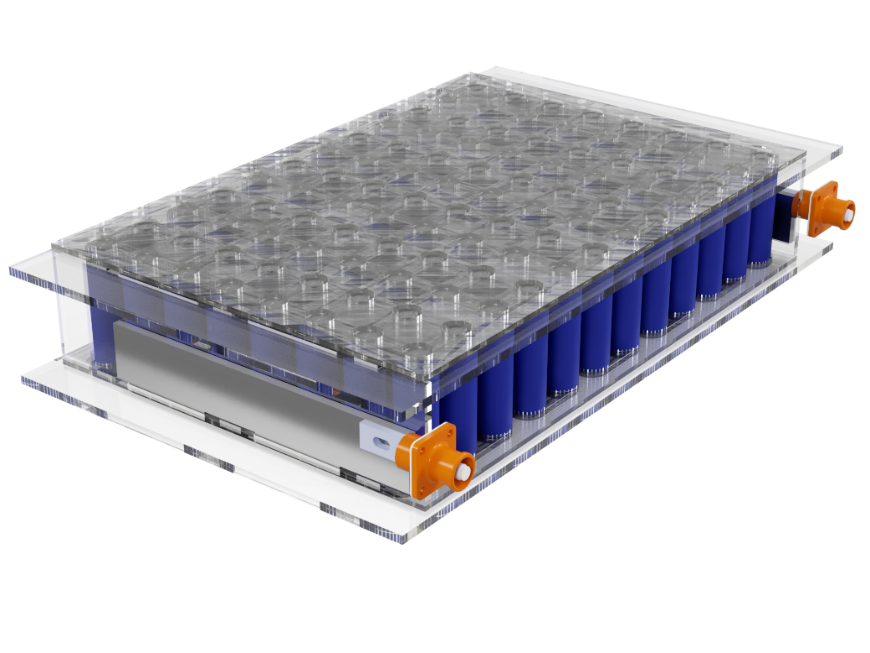
\includegraphics[height=5cm]{cont-mod-mic.png}
            \caption{Microrrede.}
            \label{fig:cont-mod-mic}
        \end{subfigure}
        %\hspace*{\fill}
        \begin{subfigure}{0.48\linewidth}
            \centering
            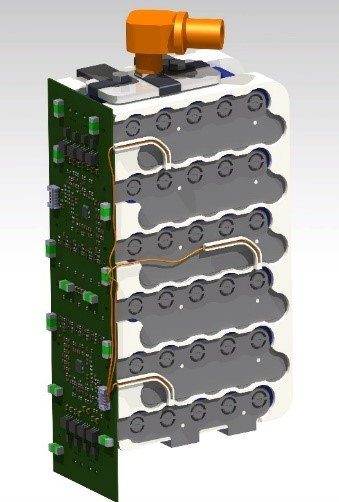
\includegraphics[height=5cm]{cont-mod-vee.jpg}
            \caption{Veículo elétrico.}
            \label{fig:cont-mod-vee}
        \end{subfigure}
        \caption{Rederização dos projetos dos módulos.}
        \label{fig:cont-mods}
    \end{figure}

    Assim como o projeto dos módulos, a montagem global dos sistemas partiu de conceitos diferentes. No sistema da microrrede o foco foi a facilidade de manutenção e instalação do sistema, assim, se optou pelo uso de racks para servidores (figura \ref{fig:cont-mod-mic}). Já o container do projeto do veículo elétrico precisou ser feito de acordo com as dimensões do chassi do carro e do posicionamento de outros componentes (figura \ref{fig:cont-mod-vee}).

    \begin{figure}[!htb]
        \centering
        \begin{subfigure}{0.48\linewidth}
            \centering
            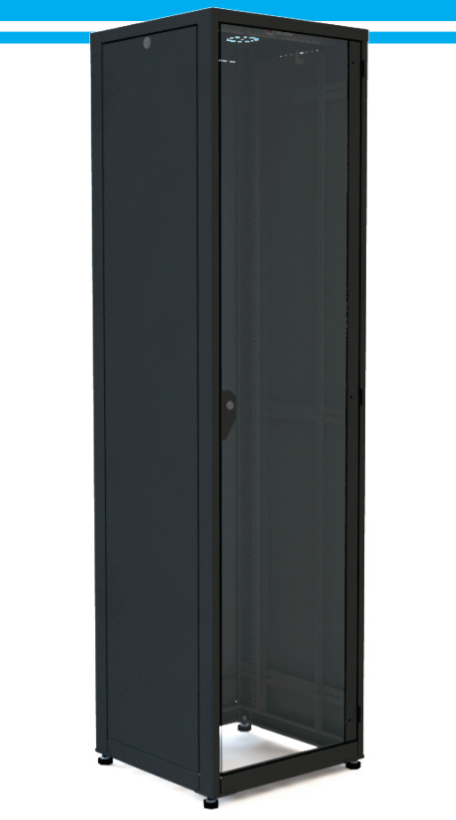
\includegraphics[height=5cm]{cont-mic.png}
            \caption{Modelo de rack utilizado de container para sistema da microrrede (disponível em: http://www.coretlc.com.br/).}
            \label{fig:cont-mod-mic}
        \end{subfigure}
        %\hspace*{\fill}
        \begin{subfigure}{0.48\linewidth}
            \centering
            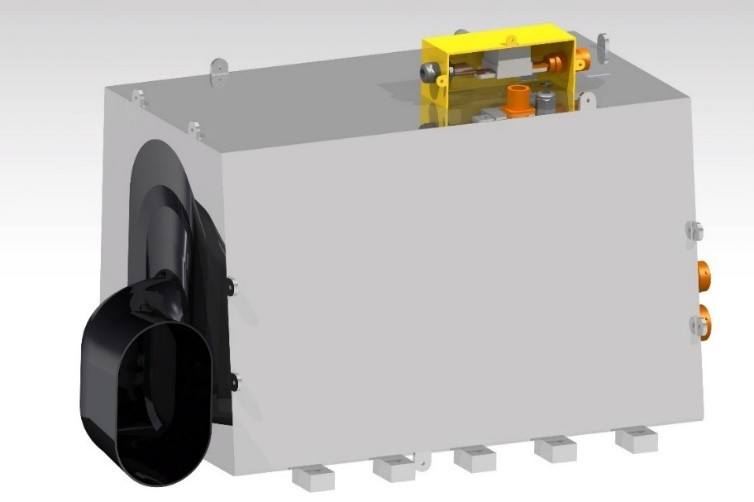
\includegraphics[height=5cm]{cont-vee.jpg}
            \caption{Rederização do container completo do veículo elétrico.}
            \label{fig:cont-mod-vee}
        \end{subfigure}
        \caption{Containeres utilizados}
        \label{fig:conts}
    \end{figure}

%=====================================================

\section{Conexões, plugs de manutenção e HVD}

    São o grupo de todas as conexões elétricas de alta tensão (\textit{High Voltage – HV}) e de baixa tensão (\textit{Low Voltage – LV}) entre dois sistemas quaisquer. Plugs de manutenção são conectores específicos para a conexão de potência entre os Segmentos, no veículo, e entre packs, na microrrede. Já o \textit{HV Disconnect (HVD)} é um sistema exclusivo do veículo elétrico, sendo o elemento fisicamente removível que permite a separação de um dos polos do sistema TS. É usado em casos de emergência para prover a separação elétrica e interromper o circuito de potência do carro. Entre os requerimentos mais importantes destes sistemas estão os cuidados que se deve ter com o isolamento elétrico e na escolha dos materiais, além de padrões de cores e a proibição do uso de estanho para conexão em sistemas de potência.

    Para a escolha dos conectores a serem utilizados foi levado em conta, além de todos os requerimentos, as necessidades e particularidades de cada conexão. Dois tipos principais de conexão são utilizados no acumulador: conexões de placa para cabo e de painel para cabo. Além disso, são usados conectores de potência para a transmissão de energia entre as células e o sistema que utilizará a energia. Dez padrões diferentes de conectores foram utilizados em mais de 50 conectores por sistema.

%=====================================================

\section{Medidor de energia}

    É também um sistema exclusivo do veículo, unicamente usado para que a entidade organizadora da competição possa medir a tensão e o consumo de energia do sistema de tração (TS). Ele é provido pelo próprio organizador da competição. Para o funcionamento do medidor de energia deve ser apenas observado o que está apontado no manual dele, fornecido pela organização da competição. Sendo que no projeto de integração do sistema isso já foi observado.

%=====================================================

\section{Fusíveis e fusível principal}

    Fusíveis é o grupo de todos os dispositivos de proteção contra sobrecorrente em ambos os sistemas HV e LV. É usado para proteger os sistemas elétricos de sobrecorrente e aquecimento dos cabos e componentes, que podem levar a queimaduras e até incêndios. Já o fusível principal está posicionado no caminho principal de corrente do acumulador e tem a função de proteger cabos, conexões, o inversor (no carro) e o conversor CC-CC (na microrrede). Entre os principais requerimentos estão aspectos do correto dimensionamento e sua montagem física. 

    Na montagem do acumulador do veículo elétrico foram ainda utilizadas conexões fusíveis para cada célula em paralelo, sendo essa um recorte na chapa de níquel que faz a conexão. Já o fusível principal foi dimensionado para corrente máxima do sistema, sendo o da microrrede de 125 A e do veículo elétrico de 225 A. Eles têm também a classificação de tensão em níveis distintos, a microrrede em 650 V e o veículo elétrico em 500 V. Ambos são fusíveis de atuação rápida próprios para a proteção de dispositivos semicondutores, como conversores e inversores.

%=====================================================

\section{Relés de isolamento do acumulador (AIRs)}

    É o dispositivo de separação de ambos os polos do Acumulador, usado para separar eletricamente todo o sistema energizado da bateria com o exterior em qualquer momento de emergência ou que não esteja sendo utilizado. Dentre os requerimentos estão aspectos do dimensionamento e a necessidade de haver um por polo do acumulador.

    No caso do veículo elétrico foi escolhido o contator com a bobina mais energeticamente eficiente do mercado. Isso com a função de reduzir o tamanho da bateria de baixa tensão do carro e por consequência diminuir o peso. Os contatores utilizados na microrrede foram os mesmos usados no ano de 2019 no carro da equipe UFPR Formula, com a principal função de reduzir os custos na implantação do sistema.

%=====================================================

\section{Circuitos de pré-carga e descarga}

    O circuito de pré-carga carrega os capacitores do inversor (no carro) e do conversor CC-CC (na microrrede) antes de fechar os relés de isolamento do acumulador (AIRs) para a conexão do acumulador com o conversor. Já o circuito de descarga descarrega esses mesmos capacitores quando os AIRs são abertos. Os requerimentos mais importantes são: é necessário carregar os capacitores ate 90\% da tensão do acumulador antes dos AIRs fecharem e é necessário que a tensão dos capacitores abaixe de 60 V DC em menos de 5 s após os AIRs abrirem

    Na microrrede ambos os circuitos já estão implementados nos circuitos do conversor CC-CC, então não há necessidade de fazer no acumulador. Já no veículo elétrico esse sistema fica dentro do container. São compostos de um relé e um resistor em cada circuito, a diferenciação é feita apenas nas conexões, no tipo do relé (normalmente aberto para o circuito de pré-carga e normalmente fechado para o circuito de descarga) e na sequência de ativação. Além disso, todos os circuitos foram projetados para funcionarem de forma segura e confiável.

%=====================================================

\section{Circuito Shutdown}

    É o circuito que carrega diretamente a corrente que realiza a ativação dos Relés de isolamento do acumulador (AIRs), passando por botões, \textit{switches}, \textit{interlocks} e \textit{latches}. É usado para abrir os relés em qualquer situação de emergência ou falha de sistemas de segurança. Dentre os requerimentos mais importantes está a lista dos itens necessários, sendo esses, dentro do container, o IMD, AMS e os respectivos \textit{interlocks} dos conectores.

%=====================================================

\section{Dispositivo de monitoramento do isolamento (IMD)}

    É um dispositivo exclusivo do carro, que mede a resistência de isolamento entre o sistema de alta tensão (\textit{High Voltage System – HVS}) e o sistema de baixa tensão aterrado (\textit{Grounded Low Voltage System – GLVS}). É usado para abrir o Circuito Shutdown em qualquer momento que houver falha de isolamento, que representaria risco para outros sistemas do carro e qualquer pessoa próxima ao expor eles à alta tensão (HV). Nos requerimentos já está definido o modelo a ser utilizado, restando o trabalho de fazer o correto dimensionamento dos seus parâmetros, que foram feitos para manter o tempo máximo para ativação abaixo do indicado nos requerimentos.

%=====================================================

\section{Sistema de gerenciamento do acumulador (AMS)}

    O sistema de gerenciamento do acumulador, conhecido por AMS ou BMS, mede e monitora todos os parâmetros das células dentro do Acumulador, mantendo-as na região de operação indicada pela fabricante e listadas nos requerimentos. É usado para medir a tensão, corrente e temperatura das células, mantendo comunicação com os usuários (inversor, conversor CC-CC, piloto ou operador do sistema) e tendo a capacidade de abrir o Circuito \textit{Shutdown} em casos de emergência. Dentre os requerimentos estão vários aspectos de projetos de PCB para alta tensão, cuidados nas conexões e a listagem dos parâmetros que devem ser verificados.

    Como apresentado na discussão sobre segurança de células de íons de lítio, o AMS é o principal sistema responsável pelo correto funcionamento do acumulador. No projeto da microrrede foi utilizado um modelo comercial, o Orion BMS 2. Este é um sistema centralizado e que conta com medições de tensão, corrente e temperatura, além de fazer a estimativa de estado de carga das células e outros parâmetros de forma muito confiável. Já no veículo elétrico, o projeto de um BMS foi feito inteiro pela equipe UFPR Formula. Este tinha por função ser mais compacto e flexível que um sistema comercial. Assim, foi possível que o projeto do BMS se integrasse no projeto dos módulos do acumulador, aumentando a confiabilidade das medições e diminuindo a quantidade de cabos. Cada placa de medição conta com a capacidade de medir a tensão e temperatura de 12 células em série, os dados são então mandados para um microcontrolador central via comunicação SPI isolada. No microcontrolador são feitas as estimativas de estado de carga e os cálculos para limitação de corrente, além da comunicação externa com sistemas de telemetria, com o inversor e com o carregador.

%=====================================================

\section{Carregador e circuito \textit{Shutdown} de carga}

    É o dispositivo usado para prover energia elétrica com a função de carregar as células do Acumulador. Pelo fato de o conversor CC-CC já realizar essa função na microrrede, este é um sistema exclusivo do carro. Já o circuito \textit{Shutdown} de carga é similar ao Circuito \textit{Shutdown}, mas é usado no momento da carga, por isso é também um sistema exclusivo do carro. Todos os requerimentos acima continuam válidos para o momento da carga, além disso, é necessário que o carregador tenha certificação de padrão reconhecido, no caso, no modelo utilizado, o CE.

    O modelo usado foi o mesmo utilizado nos últimos anos no veículo elétrico, mas dessa vez, para fazer a carga os segmentos são separados, assim, um carregador de baixa tensão (máximo 99 V do modelo utilizado) pode realizar a carga de um acumulador com tensão bem superior. Essa escolha se deve principalmente pelo fato do sistema de carga ser um componente muito caro, e como medida de redução de custos foi utilizado o mesmo que já havia sido adquirido.